\documentclass[12pt]{article}
\usepackage{array, bm, geometry, hyperref, enumerate, multirow, amsmath, color, graphics, float, rotating}
\geometry{a4paper, top=1cm, bottom=2cm, left=2cm, right=2cm}
\usepackage[table]{xcolor}
\newcommand{\code}[1]{\texttt{#1}}                      % type font
\parindent = 0.5cm
\title{Na\"ive Bayes Classification}
\author{Stu Field}
\date{}   % no date


\begin{document}
\maketitle


\section{Bayes' Rule}

\begin{equation}
	P(\theta | Data) = \frac{P(Data | \theta) \times P(\theta)}{P(Data)}
\end{equation}


\section{Bayes Classifier}

\begin{eqnarray*}
	\text{odds ratio} &=& \frac{P(x=c_1 | Data)}{P(x=c_2 | Data)} = \frac{P(Data | x=c_1) \cdot P(x=c_1)}{P(Data | x=c_2) \cdot P(x=c_2)} \\
	log(\text{odds}) &=& log\Bigg(\frac{P(Data | x=c_1)}{P(Data | x=c_2)} \cdot \frac{P(x=c_1)}{P(x=c_2)}\Bigg) \\
	log(\text{odds}) &=& log\bigg(\frac{P(Data | x=c_1)}{P(Data | x=c_2)}\bigg) + 
			log\bigg(\frac{P(x=c_1)}{P(x=c_2)}\bigg)
\end{eqnarray*}



\section{Bayes In Practice}

\begin{eqnarray*}
	\frac{P(Data | x=c_1)}{P(Data | x=c_2)} &=& 
		\frac{P(A_1=a_1, A_2=a_2,\dots,A_n=a_n|x=c_1)}
		 {P(A_1=a_1,A_2=a_2,\dots,A_n=a_n|x=c_2)} \\
		 \\
		&=& \frac{P(A_1=a_1|x=c_1) P(A_1=a_1|x=c_1),\dots,P(A_n=a_n|x=c_1)} 
		{P(A_1=a_1|x=c_2) P(A_1=a_1|x=c_2),\dots,P(A_n=a_n|x=c_2)} \\
		\\ \\ \\ 
	log\Bigg(\frac{P(Data | x=c_1)}{P(Data | x=c_2)}\Bigg) &=& 
			log\Bigg(\frac{P(A_1=a_1|x=c_1)}{P(A_1=a_1|x=c_2)}\Bigg) + \\
			\\
			&& log\Bigg(\frac{P(A_2=a_2|x=c_1)}{P(A_2=a_2|x=c_2)}\Bigg) + \dots + 
			log\Bigg(\frac{P(A_n=a_n|x=c_1)}{P(A_n=a_n|x=c_2)}\Bigg)
\end{eqnarray*}


\newpage

Therefore, putting together gives,

\begin{eqnarray*}
	log(\text{odds}) &=& log\Bigg(\frac{P(A_1=a_1|x=c_1)}{P(A_1=a_1|x=c_2)}\Bigg) + 
			log\Bigg(\frac{P(A_2=a_2|x=c_1)}{P(A_2=a_2|x=c_2)}\Bigg) + \dots \\ \\
			&& + log\Bigg(\frac{P(A_n=a_n|x=c_1)}{P(A_n=a_n|x=c_2)}\Bigg) + 
			log\bigg(\frac{P(x=c_1)}{P(x=c_2)}\bigg)
\end{eqnarray*}


where,

\begin{equation*}
			log\bigg(\frac{P(x=c_1)}{P(x=c_2)}\bigg)
\end{equation*}

is the Bayesian prior and is typically set to zero (unless known previously).


\subsection{Calculation of the Terms}

\begin{figure}[H]
	\centering
	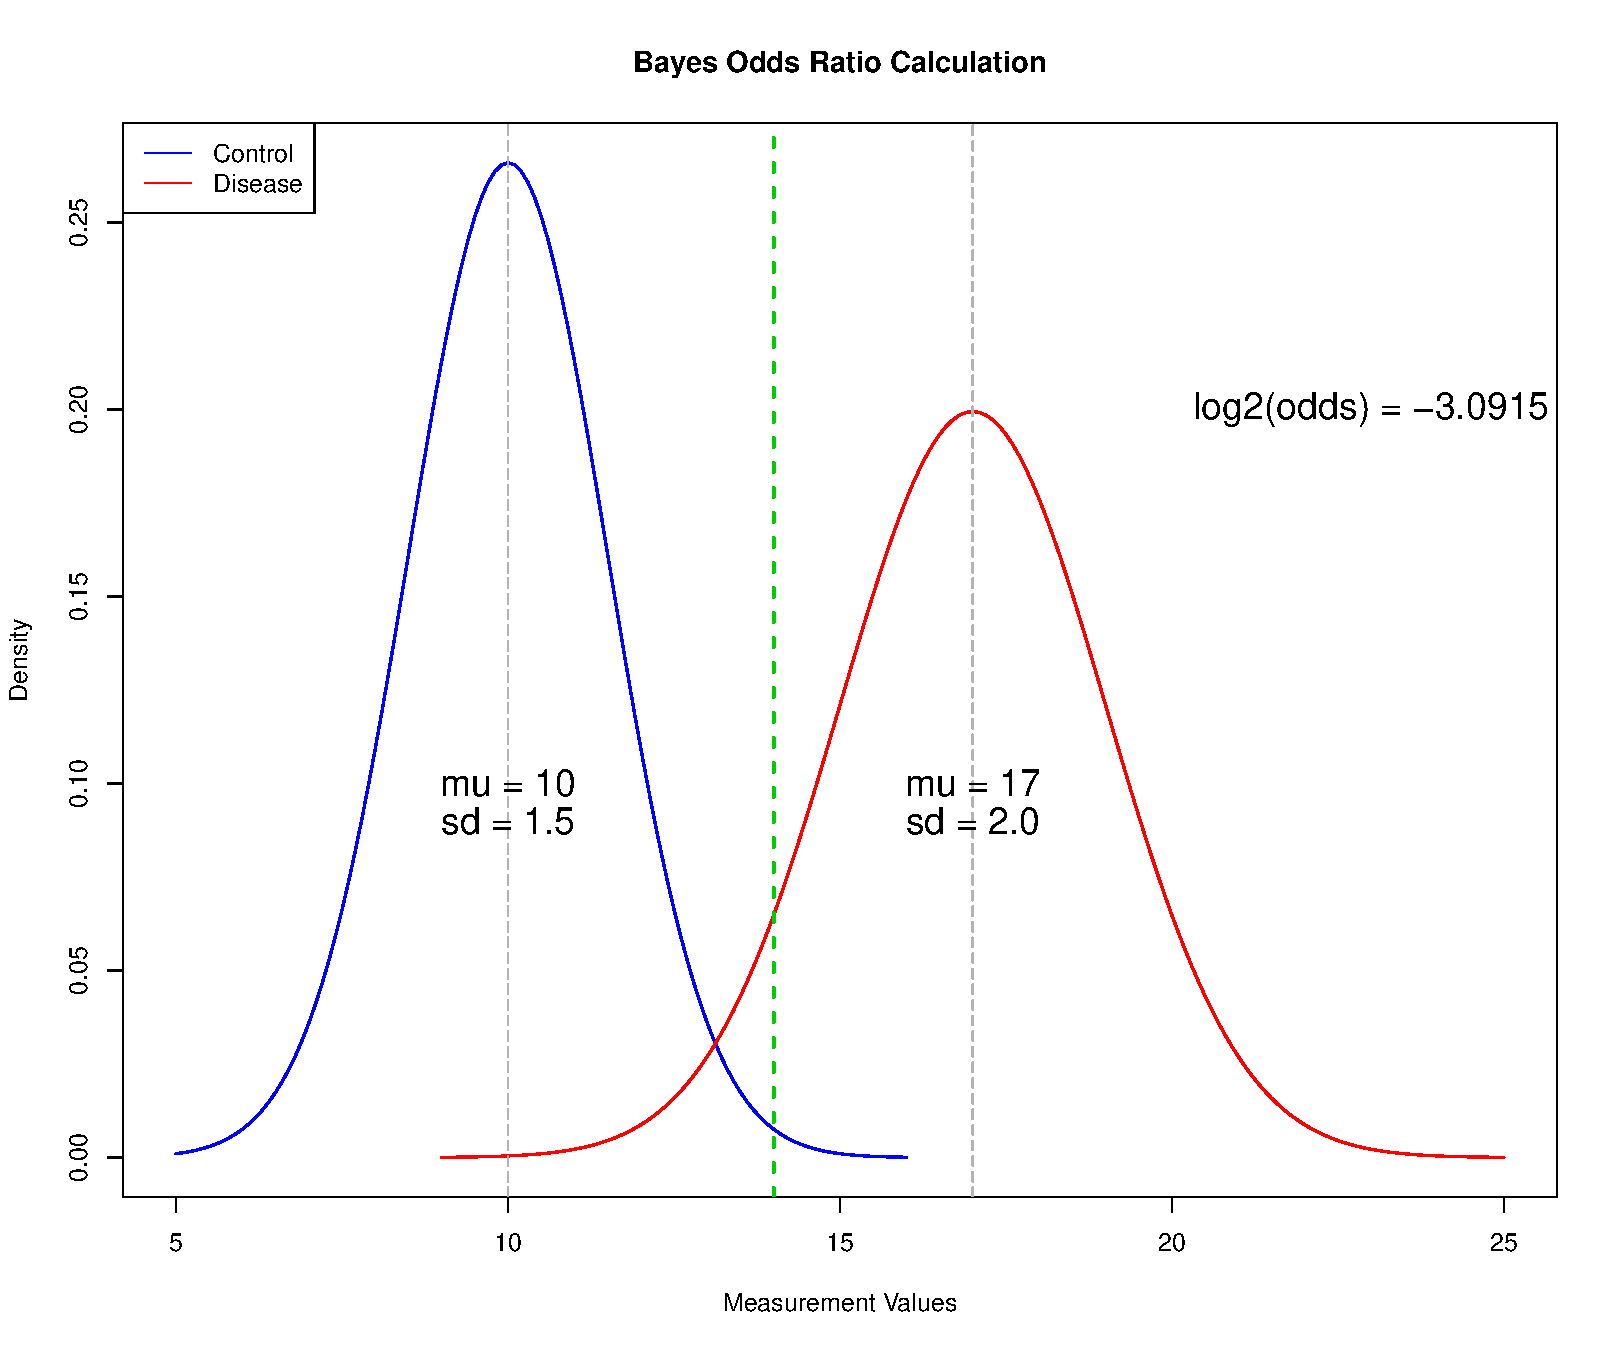
\includegraphics[width=0.8\textwidth]{plots/bayes_distn.pdf}
  \caption{PDFs of the a theoretical control population (blue) and disease population (red) for a single analyte. The population estimates are shown and the green line represents a sample value of 14. The odds ratio is the probability of control given the sample value over the probability of disease given the sample (\code{dnorm(14, 10, 1.5) / dnorm(14, 17, 2)}).}
\end{figure}


\def \hzline{\rule[0mm]{\textwidth}{1pt}}
\vfill \noindent \hzline \\ \centering{\textbf{Last updated:} \today}

\end{document}

